\documentclass[12pt,a4paper]{article}

\newcommand{\TETELNUMBER}{15}
\newcommand{\TETELTITLE}{Öröklődés, polimorfizmus, absztrakt osztály és interfész}
\newcommand{\TETELSHORTTITLE}{Öröklődés és polimorfizmus}

\newcommand{\ZVTetelsorDataOnly}{}
\newcommand{\ZVTetelOne}{Adatok, adattípusok, adatműveletek és adatstruktúrák. Szám adattípus. Számrendszerek, konverziók. A logikai, halmaz, karakter, sztring absztrakt adattípusok és realizációjuk. A tömb (vektor, mátrix), rekord absztrakt adattípusok.}
\newcommand{\ZVTetelTwo}{Az algoritmus. Iteratív és rekurzív algoritmus. A számítógépes memória. Adat és program. Verem és procedúra. Az algoritmus lejegyzése. A folyamatábra és a pszeudokód. Elemi algoritmusok.}
\newcommand{\ZVTetelThree}{Strukturált programozás. Programgráf, valódi program, vezérlőgráf lebontása, strukturált program és annak formulája. Strukturált programgráf kialakítása, struktogram. Ciklikus bonyolultság és egyéb bonyolultsági tételek.}
\newcommand{\ZVTetelFour}{Számelméleti algoritmusok. Legnagyobb közös osztó, euklideszi és kibővített euklideszi algoritmus, lineáris kongruencia egyenletek. Multiplikatív inverz, moduláris hatványozás, Fermat prímteszt. RSA.}
\newcommand{\ZVTetelFive}{Rendezések: Beszúró rendezés. Az ,,Oszd meg és uralkodj!'' elv. Összefésülő rendezés. Gyors rendezés. Buborék rendezés. Shell rendezés. Minimum kiválasztásos rendezés. Négyzetes rendezés. Lineáris idejű rendezések: leszámláló rendezés, számjegyes rendezés. Időelemzéseik. Az összehasonlító rendezések időtétele.}
\newcommand{\ZVTetelSix}{Gráfalgoritmusok. Szélességi keresés. Mélységi keresés. Topologikus rendezés. Optimumfeladatok fákon (minimális feszítőfák, Kruskal- és Prim-algoritmus). Legrövidebb utak meghatározása (Dijkstra-algoritmus, Bellman--Ford-algoritmus, Floyd--Warshall-algoritmus).}
\newcommand{\ZVTetelSeven}{A párhuzamos algoritmusok alapfogalmai, PRAM modell, hatékonysági mértékek (munka, költség, gyorsítás, hatékonyság). Párhuzamos végrehajtás ábrázolási módjai. Komplexitás becslése, párhuzamos komplexitás. Amdahl törvénye. Pipeline párhuzamosítás, Lost update probléma bemutatása és megoldása.}
\newcommand{\ZVTetelEight}{Aggregáció, redukció, prefixszámítás párhuzamosítási lehetőségei. \texttt{CREW\_PREFIX}, \texttt{EREW\_PREFIX} és \texttt{OPTIMAL\_PREFIX} algoritmusok bemutatása. Összefésülő rendezés párhuzamosítási módja.}
\newcommand{\ZVTetelNine}{A busz, gyűrű, rács, tórusz, hiperkocka és fa topológiák bemutatása, csomópontok közötti távolságok jellemzése. A CSP, Publish--Subscribe és az Aktor modell. Az aszinkron programozás elemei: async, await kulcsszavak használata, coroutine-ok.}
\newcommand{\ZVTetelTen}{A Turing-gép fogalma, működése. A RAM-gép. Boole-függvények és logikai hálózatok.}
\newcommand{\ZVTetelEleven}{Algoritmikus eldönthetőség. Church-tézis. Rekurzív és rekurzívan felsorolható nyelvek, rekurzív illetve parciálisan rekurzív függvények. Nevezetes nyelvek (Az R, Re, coR, coRE nyelvosztályok és ezek kapcsolata) és bonyolultságuk. Algoritmikusan eldönthetetlen problémák. Polinomiális idejű algoritmusok.}
\newcommand{\ZVTetelTwelve}{Nemdeterminisztikus Turing-gépek, az NP és a coNP nyelvosztály. Példák NP-beli nyelvekre. A tanú-tétel. Nemdeterminisztikus algoritmusok bonyolultsága. NP-teljesség, Cook-tétel. Néhány NP-teljes probléma, Cook--Levin-tétel.}
\newcommand{\ZVTetelThirteen}{A Java programozási nyelv története, alapvető jellemzői. Egy Java program szerkezete (csomagok és fordítási egységek). Az objektumorientált programtervezés alapelveinek felsorolása. Objektumok tárolása és élettartama. Szemétgyűjtő mechanizmus. Kivételkezelés.}
\newcommand{\ZVTetelFourteen}{Az egységbezárás és az információrejtés objektumorientált alapelvek megvalósítása. Osztálydefiníció és példányosítás. Osztályszintű és példányszintű tagok, konstansok. Hozzáférési kategóriák és használatuk. Hivatkozás az osztály tagjaira.}
\newcommand{\ZVTetelFifteen}{Az öröklődés és a polimorfizmus objektumorientált alapelvek megvalósítása. Öröklődés szabályai, metódusok túlterhelése és felüldefiniálása. A referencia statikus és dinamikus típusa. Absztrakt osztály és interfész szerepe, összehasonlítása.}
\newcommand{\ZVTetelSixteen}{Az operációs rendszerbeli folyamat (processz) fogalma. Folyamatkontextus. A fonál (szál) fogalma. A processzállapotok, állapotváltások, processz futási módok. Taszk- és fonálállapotok, állapotátmenetek.}
\newcommand{\ZVTetelSeventeen}{A memóriamenedzselés feladatai. Memória mint erőforrás. Címleképzés fajtái. Lapozós virtuális memóriamenedzselés működése. Allokálás, nyilvántartás, címleképzés. Laphiba fogalma, kezelése, kilapozási stratégiák. Előnyök, hátrányok.}
\newcommand{\ZVTetelEighteen}{Fájlrendszer-megvalósítási feladatok. Jegyzékszerkezetek. Szabadblokk-menedzselési lehetőségek. Fájlattribútum-rögzítési lehetőségek (ezen belül a fájltestet képező blokkok rögzítési lehetőségei).}
\newcommand{\ZVTetelNineteen}{Relációs adatmodell, relációs struktúra és integritási feltételek. ER modell elemei jelentése és jelölése. Az ER modell konverziója relációs modellre. Relációs adatmodell műveleti része, relációs algebra.}
\newcommand{\ZVTetelTwenty}{Az SQL szabvány relációs adatbázis kezelő nyelv bemutatása, a DDL (objektum létrehozás, megszüntetés és szerkezet módosítás), DML (rekord felvitel, törlés és módosítás), DCL és a SELECT utasítások áttekintése és használata. Beágyazott SELECT használata. A relációs algebra műveleteinek megvalósítása SQL-ben.}
\newcommand{\ZVTetelTwentyOne}{Adatkezelés és adatbáziskezelés alapfogalmai, fileszervezési módszerek, B-fa index; adatbázis architektúra; A normalizálás szerepe a relációs adatbázis kezelésben. Redundancia oka és a megszüntetés lépései. Normálformák. Dekompozíció célja és szabályai, tételei.}
\newcommand{\ZVTetelTwentyTwo}{Számítógép-hálózatokhoz kötődő alapfogalmak és az ISO--OSI hivatkozási modell: topológia és méret szerinti osztályozásuk. Kapcsolástechnika szerinti osztályozásuk (vonalkapcsolás, üzenetkapcsolás, csomagkapcsolás és virtuális vonalkapcsolás). Az ISO--OSI hivatkozási modell szerkezete, rétegei és azok főbb funkciói.}
\newcommand{\ZVTetelTwentyThree}{A számítógép-hálózatok ISO--OSI hivatkozási modell adatkapcsolati rétegének közeghozzáférési alrétege: A főbb csatorna-megosztási osztályok (statikus-dinamikus, dinamikus versengő-determinisztikus) bemutatása és azok összevetése. Az IEEE 802.3 és az Ethernet (CSMA/CD) keretformátum, MAC címek, támogatott közegek és sebességek bemutatása, működés duplex csatorna esetén. Az IEEE 802.11 WLAN általános felépítése, az Access Point (AP) főbb funkciói. Az alkalmazott közeghozzáférési módszer (CSMA/CA), Distributed Coordination Function (DCF) és Point Coordination Function (PCF) üzemmódok.}
\newcommand{\ZVTetelTwentyFour}{A TCP/IP protokollszövet és az Internet. Az Internet hivatkozási modell (DoD) és az ISO--OSI hivatkozási modell összevetése. A TCP/IP protokollszövet főbb részei (ARP, RARP, IP, ICMP, TCP, UDP) és azok funkciói. Az internetes címzés és címosztályok: IPv4-címosztályok, maszk, subnet, supernet, osztály nélküli címzés (CIDR -- Classless Inter-Domain Routing) és változó alhálózat-méretek (VLSM -- Variable Length Subnet Mask), címek kiosztása, lokális címek és címfordítás (NAT). IPv6-címek, IPv6-címtípusok (unicast, multicast, anycast; link local, unique local, aggregatable global unicast address).}
\newcommand{\ZVTetelTwentyFive}{Szoftvertechnológia és a szoftverfolyamat fogalma. A szoftverfolyamat-fázisok részletes bemutatása: szoftverspecifikáció, tervezés, implementáció, validáció és evolúció. Az evolúciós modell ismertetése.}
\newcommand{\ZVTetelTwentySix}{Szoftverkövetelmény fogalma és osztályozásai. Követelmények általános problémái. Követelményfeltárás és -elemzés folyamata. Vezérlési stílusok.}
\newcommand{\ZVTetelTwentySeven}{UML diagramok bemutatása: Use case és osztálydiagram. A szekvenciadiagram. Komponensdiagram.}

\newcommand{\ZVTetelKiiras}[1]{%
  \ifcase#1\relax
  \or \ZVTetelOne
  \or \ZVTetelTwo
  \or \ZVTetelThree
  \or \ZVTetelFour
  \or \ZVTetelFive
  \or \ZVTetelSix
  \or \ZVTetelSeven
  \or \ZVTetelEight
  \or \ZVTetelNine
  \or \ZVTetelTen
  \or \ZVTetelEleven
  \or \ZVTetelTwelve
  \or \ZVTetelThirteen
  \or \ZVTetelFourteen
  \or \ZVTetelFifteen
  \or \ZVTetelSixteen
  \or \ZVTetelSeventeen
  \or \ZVTetelEighteen
  \or \ZVTetelNineteen
  \or \ZVTetelTwenty
  \or \ZVTetelTwentyOne
  \or \ZVTetelTwentyTwo
  \or \ZVTetelTwentyThree
  \or \ZVTetelTwentyFour
  \or \ZVTetelTwentyFive
  \or \ZVTetelTwentySix
  \or \ZVTetelTwentySeven
  \fi
}

\newcommand{\ZVTetelsorList}{%
\begin{enumerate}[leftmargin=7mm,label=\arabic*.,itemsep=2pt,topsep=2pt,parsep=0pt]
  \item \ZVTetelOne
  \item \ZVTetelTwo
  \item \ZVTetelThree
  \item \ZVTetelFour
  \item \ZVTetelFive
  \item \ZVTetelSix
  \item \ZVTetelSeven
  \item \ZVTetelEight
  \item \ZVTetelNine
  \item \ZVTetelTen
  \item \ZVTetelEleven
  \item \ZVTetelTwelve
  \item \ZVTetelThirteen
  \item \ZVTetelFourteen
  \item \ZVTetelFifteen
  \item \ZVTetelSixteen
  \item \ZVTetelSeventeen
  \item \ZVTetelEighteen
  \item \ZVTetelNineteen
  \item \ZVTetelTwenty
  \item \ZVTetelTwentyOne
  \item \ZVTetelTwentyTwo
  \item \ZVTetelTwentyThree
  \item \ZVTetelTwentyFour
  \item \ZVTetelTwentyFive
  \item \ZVTetelTwentySix
  \item \ZVTetelTwentySeven
\end{enumerate}%
}


\newcommand{\tetelsorrow}[2]{\textbf{#1.} & #2\tabularnewline}

\newcommand{\tetelsorpageone}{%
\begin{tabularx}{\textwidth}{|>{\raggedleft\bfseries}p{8mm}@{\hspace{5mm}}>{\raggedright\arraybackslash}X|}
\hline
\tetelsorrow{1}{\ZVTetelOne}
\tetelsorrow{2}{\ZVTetelTwo}
\tetelsorrow{3}{\ZVTetelThree}
\hline
\tetelsorrow{4}{\ZVTetelFour}
\tetelsorrow{5}{\ZVTetelFive}
\tetelsorrow{6}{\ZVTetelSix}
\hline
\tetelsorrow{7}{\ZVTetelSeven}
\tetelsorrow{8}{\ZVTetelEight}
\tetelsorrow{9}{\ZVTetelNine}
\hline
\tetelsorrow{10}{\ZVTetelTen}
\tetelsorrow{11}{\ZVTetelEleven}
\tetelsorrow{12}{\ZVTetelTwelve}
\hline
\end{tabularx}%
}

\newcommand{\tetelsorpagetwo}{%
\begin{tabularx}{\textwidth}{|>{\raggedleft\bfseries}p{8mm}@{\hspace{5mm}}>{\raggedright\arraybackslash}X|}
\hline
\tetelsorrow{13}{\ZVTetelThirteen}
\tetelsorrow{14}{\ZVTetelFourteen}
\tetelsorrow{15}{\ZVTetelFifteen}
\hline
\tetelsorrow{16}{\ZVTetelSixteen}
\tetelsorrow{17}{\ZVTetelSeventeen}
\tetelsorrow{18}{\ZVTetelEighteen}
\hline
\tetelsorrow{19}{\ZVTetelNineteen}
\tetelsorrow{20}{\ZVTetelTwenty}
\tetelsorrow{21}{\ZVTetelTwentyOne}
\hline
\tetelsorrow{22}{\ZVTetelTwentyTwo}
\tetelsorrow{23}{\ZVTetelTwentyThree}
\tetelsorrow{24}{\ZVTetelTwentyFour}
\hline
\tetelsorrow{25}{\ZVTetelTwentyFive}
\tetelsorrow{26}{\ZVTetelTwentySix}
\tetelsorrow{27}{\ZVTetelTwentySeven}
\hline
\end{tabularx}%
}

\ifdefined\ZVTetelsorDataOnly
\expandafter\endinput
\fi

\documentclass[10pt,a4paper]{article}
\newcommand{\ZVHEADERLEFT}{Záróvizsga tételek}
\newcommand{\ZVHEADERRIGHT}{Programtervező informatikus BSc}
\usepackage{fontspec}
\usepackage{geometry}
\usepackage{microtype}
\usepackage{xcolor}
\usepackage{amsmath,amssymb,mathtools}
\usepackage{booktabs,longtable,tabularx,array,multirow}
\usepackage{enumitem}
\usepackage{hyperref}
\usepackage{fancyhdr}
\usepackage{titlesec}
\usepackage{listings}
\usepackage[most]{tcolorbox}
\usepackage{tikz}
\usetikzlibrary{positioning,shapes.geometric,shapes.misc,arrows.meta,decorations.pathreplacing}
\usepackage{caption}

\setlength{\headheight}{16pt}
\emergencystretch=2em
\renewcommand{\contentsname}{Tartalom}

% Fontbeallitasok: ha a DejaVu fontok nincsenek telepitve,
% akkor automatikusan a MiKTeX/TeX Live alap Latin Modern fontjaira valtunk.
\IfFontExistsTF{DejaVu Serif}{\setmainfont{DejaVu Serif}}{\setmainfont{Latin Modern Roman}}
\IfFontExistsTF{DejaVu Sans}{\setsansfont{DejaVu Sans}}{\setsansfont{Latin Modern Sans}}
\IfFontExistsTF{DejaVu Sans Mono}{\setmonofont{DejaVu Sans Mono}}{\setmonofont{Latin Modern Mono}}

\geometry{left=25mm,right=25mm,top=24mm,bottom=27mm}

\hypersetup{
  colorlinks=true,
  linkcolor=blue!45!black,
  urlcolor=blue!55!black,
  pdftitle={Zarovizsga tetel},
  pdfauthor={Baba Levente - tanulasi segedanyag}
}

\definecolor{accent}{HTML}{1F4E79}
\definecolor{lightaccent}{HTML}{EAF2F8}
\definecolor{warnbg}{HTML}{FFF4E5}
\definecolor{codebg}{HTML}{F7F7F7}

\tikzset{
  flow/.style={draw, rounded corners, align=center, minimum width=21mm, minimum height=8mm, fill=lightaccent},
  pred/.style={draw, diamond, aspect=2, align=center, inner sep=1pt, fill=warnbg},
  merge/.style={draw, circle, inner sep=1.2pt, fill=black!8},
  terminator/.style={draw, rounded corners=4mm, align=center, minimum width=20mm, minimum height=8mm, fill=black!5},
  arrow/.style={->, >=stealth, thick},
  zvflowstart/.style={draw, rounded rectangle, minimum width=2.3cm, minimum height=0.7cm, align=center},
  zvflowprocess/.style={draw, rectangle, minimum width=2.7cm, minimum height=0.7cm, align=center},
  zvflowdecision/.style={draw, diamond, aspect=2.2, minimum width=2.8cm, minimum height=0.8cm, align=center}
}


\titleformat{\section}{\Large\bfseries\sffamily\color{accent}}{\thesection.}{0.6em}{}
\titleformat{\subsection}{\large\bfseries\sffamily\color{accent}}{\thesubsection.}{0.6em}{}
\titleformat{\subsubsection}{\normalsize\bfseries\sffamily\color{accent}}{\thesubsubsection.}{0.6em}{}

\setlist[itemize]{topsep=3pt,itemsep=2pt,parsep=0pt,leftmargin=1.4em}
\setlist[enumerate]{topsep=3pt,itemsep=2pt,parsep=0pt,leftmargin=1.6em}
\setlength{\parindent}{0pt}
\setlength{\parskip}{6pt}
\renewcommand{\arraystretch}{1.25}
\newcolumntype{L}[1]{>{\raggedright\arraybackslash}p{#1}}
\renewcommand{\tabularxcolumn}[1]{>{\raggedright\arraybackslash}p{#1}}

\providecommand{\ZVHEADERLEFT}{\TETELNUMBER. tétel}
\providecommand{\ZVHEADERRIGHT}{\TETELSHORTTITLE}

\pagestyle{fancy}
\fancyhf{}
\lhead{\ZVHEADERLEFT}
\rhead{\ZVHEADERRIGHT}
\cfoot{\thepage}

\lstdefinelanguage{pseudocode}{
  morekeywords={IF,THEN,ELSE,WHILE,DO,FOR,TO,DOWNTO,REPEAT,UNTIL,RETURN,CALL,INPUT,OUTPUT,AND,OR,NOT,TRUE,FALSE},
  sensitive=true,
  morecomment=[l]{//}
}

\lstdefinestyle{code}{
  basicstyle=\ttfamily\small,
  backgroundcolor=\color{codebg},
  frame=single,
  rulecolor=\color{black!15},
  columns=fullflexible,
  keepspaces=true,
  breaklines=true,
  tabsize=2,
  showstringspaces=false,
  numbers=left,
  numberstyle=\tiny\color{black!55},
  numbersep=7pt,
  xleftmargin=2.2em,
  framexleftmargin=1.7em,
  captionpos=b
}

\lstdefinestyle{pseudo}{
  style=code,
  language=pseudocode,
  keywordstyle=\bfseries\color{accent!85!black},
  commentstyle=\itshape\color{black!55}
}

\lstdefinestyle{csource}{
  style=code,
  language=C,
  keywordstyle=\bfseries\color{accent!85!black},
  commentstyle=\itshape\color{black!55},
  stringstyle=\color{orange!70!black}
}

\lstset{style=code}
\renewcommand{\lstlistingname}{Kódrészlet}
\renewcommand{\lstlistlistingname}{Kódrészletek}
\newcommand{\zvcode}[2][]{\lstinputlisting[style=code,#1]{#2}}
\newcommand{\zvpseudocode}[2][]{\lstinputlisting[style=pseudo,#1]{#2}}
\newcommand{\zvccode}[2][]{\lstinputlisting[style=csource,#1]{#2}}

\newtcolorbox{summarybox}{
  enhanced,
  colback=lightaccent,
  colframe=accent!70!black,
  arc=2mm,
  boxrule=0.5pt,
  left=2mm,right=2mm,top=1mm,bottom=1mm
}

\newtcolorbox{warningbox}{
  enhanced,
  colback=warnbg,
  colframe=orange!70!black,
  arc=2mm,
  boxrule=0.5pt,
  left=2mm,right=2mm,top=1mm,bottom=1mm
}

\newcommand{\adt}[2]{\ensuremath{#1=(#2)}}
\newcommand{\set}[1]{\ensuremath{\{#1\}}}
\newcommand{\code}[1]{\texttt{#1}}
\newcommand{\base}[2]{\ensuremath{#1_{(#2)}}}
\newcommand{\addr}{\ensuremath{@}}


\providecommand{\TETELKIIRAS}{\TETELTITLE. \TETELTOPIC}
\providecommand{\ZVAUTHOR}{Baba Levente}
\providecommand{\ZVYEAR}{2026}
\providecommand{\ZVAID}{ChatGPT segítségével}

\newcommand{\makezvtitle}{%
\begin{titlepage}
  \centering
  \vspace*{18mm}
  {\Large\sffamily Programtervező Informatikus BSc\par}
  \vspace{1mm}
  {\large\sffamily \ZVYEAR-os záróvizsga tételek\par}
  \vspace{15mm}
  {\Huge\bfseries\sffamily \TETELNUMBER. tétel\par}
  \vspace{5mm}
  {\LARGE\bfseries\sffamily \TETELTITLE\par}
  \vspace{10mm}
  \begin{summarybox}
    \textbf{Tételkiírás:} \TETELKIIRAS
  \end{summarybox}
  \vfill
  {\large Készítette: \textbf{\ZVAUTHOR}\par}
  \vspace{2mm}
  {\large \ZVAID\par}
\end{titlepage}%
}

\newcommand{\zvfrontmatter}{%
  \sloppy
  \makezvtitle
  \tableofcontents
  \newpage
}

\begin{document}
\newgeometry{left=13mm,right=13mm,top=13mm,bottom=13mm}
\pagestyle{empty}
\setlength{\tabcolsep}{2.6pt}
\renewcommand{\arraystretch}{1.08}
\begin{center}
  {\Huge\bfseries Záróvizsga tételek\par}
  \vspace{2mm}
  {\Large\itshape Programtervező informatikus BSc\par}
\end{center}
\vspace{10mm}
{\fontsize{10.5}{12.2}\selectfont
\tetelsorpageone
}
\newpage
{\fontsize{10.5}{12.2}\selectfont
\tetelsorpagetwo
}
\end{document}

\newcommand{\TETELKIIRAS}{\ZVTetelKiiras{\TETELNUMBER}}

\usepackage{fontspec}
\usepackage{geometry}
\usepackage{microtype}
\usepackage{xcolor}
\usepackage{amsmath,amssymb,mathtools}
\usepackage{booktabs,longtable,tabularx,array,multirow}
\usepackage{enumitem}
\usepackage{hyperref}
\usepackage{fancyhdr}
\usepackage{titlesec}
\usepackage{listings}
\usepackage[most]{tcolorbox}
\usepackage{tikz}
\usetikzlibrary{positioning,shapes.geometric,shapes.misc,arrows.meta,decorations.pathreplacing}
\usepackage{caption}

\setlength{\headheight}{16pt}
\emergencystretch=2em
\renewcommand{\contentsname}{Tartalom}

% Fontbeallitasok: ha a DejaVu fontok nincsenek telepitve,
% akkor automatikusan a MiKTeX/TeX Live alap Latin Modern fontjaira valtunk.
\IfFontExistsTF{DejaVu Serif}{\setmainfont{DejaVu Serif}}{\setmainfont{Latin Modern Roman}}
\IfFontExistsTF{DejaVu Sans}{\setsansfont{DejaVu Sans}}{\setsansfont{Latin Modern Sans}}
\IfFontExistsTF{DejaVu Sans Mono}{\setmonofont{DejaVu Sans Mono}}{\setmonofont{Latin Modern Mono}}

\geometry{left=25mm,right=25mm,top=24mm,bottom=27mm}

\hypersetup{
  colorlinks=true,
  linkcolor=blue!45!black,
  urlcolor=blue!55!black,
  pdftitle={Zarovizsga tetel},
  pdfauthor={Baba Levente - tanulasi segedanyag}
}

\definecolor{accent}{HTML}{1F4E79}
\definecolor{lightaccent}{HTML}{EAF2F8}
\definecolor{warnbg}{HTML}{FFF4E5}
\definecolor{codebg}{HTML}{F7F7F7}

\tikzset{
  flow/.style={draw, rounded corners, align=center, minimum width=21mm, minimum height=8mm, fill=lightaccent},
  pred/.style={draw, diamond, aspect=2, align=center, inner sep=1pt, fill=warnbg},
  merge/.style={draw, circle, inner sep=1.2pt, fill=black!8},
  terminator/.style={draw, rounded corners=4mm, align=center, minimum width=20mm, minimum height=8mm, fill=black!5},
  arrow/.style={->, >=stealth, thick},
  zvflowstart/.style={draw, rounded rectangle, minimum width=2.3cm, minimum height=0.7cm, align=center},
  zvflowprocess/.style={draw, rectangle, minimum width=2.7cm, minimum height=0.7cm, align=center},
  zvflowdecision/.style={draw, diamond, aspect=2.2, minimum width=2.8cm, minimum height=0.8cm, align=center}
}


\titleformat{\section}{\Large\bfseries\sffamily\color{accent}}{\thesection.}{0.6em}{}
\titleformat{\subsection}{\large\bfseries\sffamily\color{accent}}{\thesubsection.}{0.6em}{}
\titleformat{\subsubsection}{\normalsize\bfseries\sffamily\color{accent}}{\thesubsubsection.}{0.6em}{}

\setlist[itemize]{topsep=3pt,itemsep=2pt,parsep=0pt,leftmargin=1.4em}
\setlist[enumerate]{topsep=3pt,itemsep=2pt,parsep=0pt,leftmargin=1.6em}
\setlength{\parindent}{0pt}
\setlength{\parskip}{6pt}
\renewcommand{\arraystretch}{1.25}
\newcolumntype{L}[1]{>{\raggedright\arraybackslash}p{#1}}
\renewcommand{\tabularxcolumn}[1]{>{\raggedright\arraybackslash}p{#1}}

\providecommand{\ZVHEADERLEFT}{\TETELNUMBER. tétel}
\providecommand{\ZVHEADERRIGHT}{\TETELSHORTTITLE}

\pagestyle{fancy}
\fancyhf{}
\lhead{\ZVHEADERLEFT}
\rhead{\ZVHEADERRIGHT}
\cfoot{\thepage}

\lstdefinelanguage{pseudocode}{
  morekeywords={IF,THEN,ELSE,WHILE,DO,FOR,TO,DOWNTO,REPEAT,UNTIL,RETURN,CALL,INPUT,OUTPUT,AND,OR,NOT,TRUE,FALSE},
  sensitive=true,
  morecomment=[l]{//}
}

\lstdefinestyle{code}{
  basicstyle=\ttfamily\small,
  backgroundcolor=\color{codebg},
  frame=single,
  rulecolor=\color{black!15},
  columns=fullflexible,
  keepspaces=true,
  breaklines=true,
  tabsize=2,
  showstringspaces=false,
  numbers=left,
  numberstyle=\tiny\color{black!55},
  numbersep=7pt,
  xleftmargin=2.2em,
  framexleftmargin=1.7em,
  captionpos=b
}

\lstdefinestyle{pseudo}{
  style=code,
  language=pseudocode,
  keywordstyle=\bfseries\color{accent!85!black},
  commentstyle=\itshape\color{black!55}
}

\lstdefinestyle{csource}{
  style=code,
  language=C,
  keywordstyle=\bfseries\color{accent!85!black},
  commentstyle=\itshape\color{black!55},
  stringstyle=\color{orange!70!black}
}

\lstset{style=code}
\renewcommand{\lstlistingname}{Kódrészlet}
\renewcommand{\lstlistlistingname}{Kódrészletek}
\newcommand{\zvcode}[2][]{\lstinputlisting[style=code,#1]{#2}}
\newcommand{\zvpseudocode}[2][]{\lstinputlisting[style=pseudo,#1]{#2}}
\newcommand{\zvccode}[2][]{\lstinputlisting[style=csource,#1]{#2}}

\newtcolorbox{summarybox}{
  enhanced,
  colback=lightaccent,
  colframe=accent!70!black,
  arc=2mm,
  boxrule=0.5pt,
  left=2mm,right=2mm,top=1mm,bottom=1mm
}

\newtcolorbox{warningbox}{
  enhanced,
  colback=warnbg,
  colframe=orange!70!black,
  arc=2mm,
  boxrule=0.5pt,
  left=2mm,right=2mm,top=1mm,bottom=1mm
}

\newcommand{\adt}[2]{\ensuremath{#1=(#2)}}
\newcommand{\set}[1]{\ensuremath{\{#1\}}}
\newcommand{\code}[1]{\texttt{#1}}
\newcommand{\base}[2]{\ensuremath{#1_{(#2)}}}
\newcommand{\addr}{\ensuremath{@}}


\providecommand{\TETELKIIRAS}{\TETELTITLE. \TETELTOPIC}
\providecommand{\ZVAUTHOR}{Baba Levente}
\providecommand{\ZVYEAR}{2026}
\providecommand{\ZVAID}{ChatGPT segítségével}

\newcommand{\makezvtitle}{%
\begin{titlepage}
  \centering
  \vspace*{18mm}
  {\Large\sffamily Programtervező Informatikus BSc\par}
  \vspace{1mm}
  {\large\sffamily \ZVYEAR-os záróvizsga tételek\par}
  \vspace{15mm}
  {\Huge\bfseries\sffamily \TETELNUMBER. tétel\par}
  \vspace{5mm}
  {\LARGE\bfseries\sffamily \TETELTITLE\par}
  \vspace{10mm}
  \begin{summarybox}
    \textbf{Tételkiírás:} \TETELKIIRAS
  \end{summarybox}
  \vfill
  {\large Készítette: \textbf{\ZVAUTHOR}\par}
  \vspace{2mm}
  {\large \ZVAID\par}
\end{titlepage}%
}

\newcommand{\zvfrontmatter}{%
  \sloppy
  \makezvtitle
  \tableofcontents
  \newpage
}


\begin{document}
\zvfrontmatter
\section{A tétel lényege és vizsgaszintű vázlata}

\begin{summarybox}
A 15. tétel az objektumorientált programozás típuskapcsolatait tárgyalja. Az öröklődés segítségével általánosabb osztályból speciálisabb osztályt hozunk létre, a polimorfizmus pedig lehetővé teszi, hogy ugyanazon ősosztály vagy interfész típusú referencián keresztül különböző dinamikus típusú objektumokat kezeljünk. Ehhez kapcsolódik a metódusok túlterhelése és felüldefiniálása, a referencia statikus és dinamikus típusa, valamint az absztrakt osztály és az interfész szerepe.
\end{summarybox}

Vizsgán célszerű a következő sorrendet követni:

\begin{enumerate}
  \item röviden megfogalmazni, hogy az öröklődés az ``is-a'' jellegű specializáció eszköze;
  \item bemutatni az öröklődés Java-beli szabályait: \code{extends}, egyszeres osztályöröklés, \code{super}, konstruktorok, láthatóság;
  \item elválasztani a metódustúlterhelést és a metódusfelüldefiniálást;
  \item megmagyarázni a statikus és dinamikus típust;
  \item bemutatni, hogyan következik ebből a futásidejű polimorfizmus;
  \item definiálni az absztrakt osztályt és az interfészt;
  \item összehasonlítani az absztrakt osztályt és az interfészt;
  \item példával szemléltetni, hogy az ősosztály/interfész típusú referencia mögött eltérő objektumok állhatnak.
\end{enumerate}

A legfontosabb vizsgamondat: a referencia statikus típusa határozza meg, hogy a fordító milyen tagok használatát engedi meg, a felüldefiniált példánymetódus tényleges implementációját viszont futási időben az objektum dinamikus típusa alapján választja ki a rendszer.

\begin{center}
\begin{tabularx}{\textwidth}{L{34mm}X X}
\toprule
\textbf{Fogalom} & \textbf{Jelentése} & \textbf{Java-beli eszköz / megjegyzés} \\
\midrule
Öröklődés & Új osztály létrehozása meglévő osztály specializálásával. & \code{extends}; Java-ban osztályok között egyszeres öröklődés van, de több interfész is megvalósítható. \\
Ősosztály & Az általánosabb osztály, amely közös állapotot és viselkedést adhat. & Közös mezők, metódusok, konstruktorlogika; minden osztály közvetve a \code{Object} leszármazottja. \\
Leszármazott osztály & Az ősosztály speciálisabb változata. & Örökli az elérhető tagokat, új tagokat vehet fel, metódusokat felüldefiniálhat. \\
Polimorfizmus & Ugyanazon típusú referencia mögött többféle tényleges objektum állhat. & Őstípusú, absztrakt osztály típusú vagy interfész típusú referencia; dinamikus metóduskötés. \\
Túlterhelés & Azonos nevű metódusok eltérő paraméterlistával. & Fordítási időben dől el, hogy melyik metódusváltozat illeszkedik. \\
Felüldefiniálás & Örökölt példánymetódus új implementációja leszármazottban. & \code{@Override}; futási időben a dinamikus típus alapján választódik ki. \\
\bottomrule
\end{tabularx}

\end{center}

\section{Öröklődés az objektumorientált programozásban}

\subsection{Az öröklődés fogalma}

Az \textbf{öröklődés} olyan objektumorientált eszköz, amellyel egy meglévő, általánosabb osztályból új, speciálisabb osztályt hozunk létre. Az általánosabb osztályt ősosztálynak, alaposztálynak vagy szülőosztálynak, a speciálisabbat leszármazott osztálynak vagy gyermekosztálynak nevezzük.

Az öröklődés lényege, hogy a leszármazott osztály megkapja az ősosztály elérhető tagjait, és ezekhez új tagokat adhat hozzá, illetve bizonyos műveletek viselkedését átdefiniálhatja. Például az \code{Animal} általános állatot jelenthet, a \code{Dog} és a \code{Cat} pedig ennek speciálisabb változatai.

Az öröklődés tipikus céljai:

\begin{itemize}
  \item közös tulajdonságok és műveletek kiemelése egy közös ősosztályba;
  \item kódújrafelhasználás, mert a közös metódusokat nem kell több helyen megírni;
  \item típushierarchia kialakítása;
  \item polimorf használat lehetővé tétele;
  \item az általános és speciális viselkedés szétválasztása.
\end{itemize}

\begin{warningbox}
Az öröklődés nem egyszerű kódmásolás. Tervezési jelentése van: azt fejezi ki, hogy a leszármazott objektum az ősosztály egy speciális esete. Ha csak egy másik osztály szolgáltatásait akarjuk használni, gyakran jobb megoldás a kompozíció, vagyis amikor egy objektum egy másik objektumot adattagként tartalmaz.
\end{warningbox}

\subsection{Is-a kapcsolat és specializáció}

Az öröklődés természetes értelmezése az \textbf{is-a} kapcsolat. A \code{Dog} objektum egy \code{Animal}, ezért egy kutyát lehet állatként kezelni. Ezzel szemben ha egy \code{Car} tartalmaz egy \code{Engine} objektumot, az nem öröklődési kapcsolat, mert az autó nem motor, hanem van motorja. Ez inkább \textbf{has-a} kapcsolat, amelyet összetétellel célszerű modellezni.

A jó öröklési hierarchiában az ősosztály általános szerződést ad, a leszármazott pedig ennek megfelelően működik. Ha az ősosztály helyére behelyettesített leszármazott objektum meglepően vagy ellentmondásosan viselkedik, akkor a hierarchia valószínűleg rosszul lett megtervezve.

\subsection{Java-beli alapszintaxis}

Java-ban az osztályöröklődés kulcsszava az \code{extends}:

\[
  \code{class Dog extends Animal \{ ... \}}
\]

Ez azt jelenti, hogy a \code{Dog} osztály közvetlen ősosztálya az \code{Animal}. Java-ban egy osztálynak legfeljebb egy közvetlen ősosztálya lehet. Ha nem adunk meg ősosztályt, akkor az osztály közvetlenül vagy közvetve a \code{java.lang.Object} leszármazottja.

A \code{Object} osztályból származik több általános metódus, például a \code{toString}, az \code{equals}, a \code{hashCode} és a \code{getClass}. Ezeket szükség esetén felül lehet definiálni, például azért, hogy egy objektum szöveges megjelenítése vagy összehasonlítása a saját osztályunk szemantikájának megfelelő legyen.

\section{Az öröklődés szabályai Java-ban}

\subsection{Mit örököl a leszármazott?}

A leszármazott osztály örökli az ősosztály elérhető tagjait, de ez nem azt jelenti, hogy minden tagot közvetlenül ugyanúgy használhat. A láthatóság meghatározza, hogy a leszármazott forráskódjából mi érhető el.

Általános szabályok:

\begin{itemize}
  \item a \code{public} tagok mindenhol elérhetők, ha maga a típus is elérhető;
  \item a \code{protected} tagok az adott csomagon belül és leszármazott osztályból is elérhetők;
  \item a csomagszintű, vagyis módosító nélküli tagok csak azonos csomagból láthatók;
  \item a \code{private} tagok nem érhetők el közvetlenül a leszármazott osztály forráskódjából;
  \item a konstruktorok nem öröklődnek, de a leszármazott konstruktorának hívnia kell az ős megfelelő konstruktorát.
\end{itemize}

Fontos, hogy a \code{private} mező fizikailag része az objektumnak, ha az ősosztály definiálta, de a leszármazott csak az ősosztály publikus vagy védett metódusain keresztül férhet hozzá. Ez az információrejtés miatt lényeges.

\subsection{Konstruktorok és a \code{super} kulcsszó}

A konstruktorok nem öröklődnek. Amikor leszármazott objektum jön létre, először az ősosztály része inicializálódik, utána a leszármazott osztály saját része. Ezért a leszármazott konstruktorának közvetlenül vagy közvetve meg kell hívnia az ősosztály konstruktorát.

Ha a leszármazott konstruktorában nem szerepel explicit \code{super(...)} hívás, a fordító megpróbál egy paraméter nélküli \code{super()} hívást beszúrni. Ha az ősosztálynak nincs paraméter nélküli konstruktora, akkor a leszármazott konstruktorában kötelező explicit módon meghívni valamelyik ős-konstruktort.

A \code{super} másik szerepe, hogy az ősosztály felüldefiniált metódusára vagy elrejtett tagjára lehet vele hivatkozni:

\[
  \code{super.makeSound();}
\]

Ezt akkor használjuk, ha a leszármazott viselkedése az ős viselkedésére épül, és azt kiegészíti.

\subsection{A \code{final} szerepe öröklődésnél}

A \code{final} módosító öröklődésnél tiltó szerepet is kaphat:

\begin{itemize}
  \item \code{final class}: az osztályból nem lehet leszármazni;
  \item \code{final} metódus: a metódust nem lehet felüldefiniálni;
  \item \code{final} mező vagy lokális változó: egyszer kaphat értéket, utána nem módosítható.
\end{itemize}

Az osztály vagy metódus \code{final} jelölése akkor hasznos, ha a tervező nem akar további specializációt engedni, vagy biztosítani akarja, hogy egy metódus viselkedése ne változhasson meg leszármazott osztályban.

\subsection{Öröklődés és csatolás}

Az öröklődés erős kapcsolatot hoz létre az ősosztály és a leszármazott között. A leszármazott függ az ős publikus és védett szerződésétől, gyakran pedig az ős implementációjának részleteitől is. Emiatt az öröklődést körültekintően kell használni.

Jó használat esetén az öröklődés áttekinthető hierarchiát és polimorf felületet ad. Rossz használat esetén mély, nehezen karbantartható hierarchia alakulhat ki, ahol az ősosztály módosítása váratlanul több leszármazott működését is megváltoztatja.

\section{Metódusok túlterhelése és felüldefiniálása}

\subsection{Metódustúlterhelés}

A \textbf{metódustúlterhelés} azt jelenti, hogy ugyanazon a néven több metódust definiálunk, de eltérő paraméterlistával. A paraméterlista része a paraméterek száma, típusa és sorrendje. A visszatérési típus önmagában nem elegendő két metódus megkülönböztetésére.

Például egy \code{Logger} osztályban lehet több \code{log} metódus:

\begin{itemize}
  \item \code{log(String message)};
  \item \code{log(int value)};
  \item \code{log(Object value)}.
\end{itemize}

Túlterhelésnél a fordító választja ki, hogy az argumentumok alapján melyik metódusváltozat illeszkedik. Ezért ezt gyakran fordításidejű vagy statikus polimorfizmusnak is nevezik.

\subsection{Metódusfelüldefiniálás}

A \textbf{metódusfelüldefiniálás} azt jelenti, hogy a leszármazott osztály új implementációt ad az ősosztály egyik örökölt példánymetódusára. A metódus neve és paraméterlistája azonos, a visszatérési típus pedig azonos vagy kovariáns lehet.

Java-ban felüldefiniáláskor ajánlott az \code{@Override} annotáció használata. Ez nem kötelező a működéshez, de segít, mert a fordító hibát jelez, ha valójában nem sikerült felüldefiniálni az ős metódusát, például elírtuk a metódus nevét vagy paraméterlistáját.

A felüldefiniálás szabályai közül vizsgán különösen fontosak:

\begin{itemize}
  \item csak öröklött példánymetódus definiálható felül;
  \item a \code{private} metódus nem definiálható felül, mert nem látható örökölt metódusként;
  \item a \code{static} metódus nem felüldefiniálódik, hanem legfeljebb elrejtődik;
  \item a \code{final} metódus nem definiálható felül;
  \item a leszármazott nem szűkítheti a láthatóságot, például \code{public} metódusból nem lehet \code{protected} felüldefiniált metódus.
\end{itemize}

\begin{center}
\begin{tabularx}{\textwidth}{L{31mm}X X}
\toprule
\textbf{Szempont} & \textbf{Túlterhelés} & \textbf{Felüldefiniálás} \\
\midrule
Angol név & Overloading. & Overriding. \\
Kapcsolat & Egy osztályon belül vagy öröklési láncban is előfordulhat. & Öröklődéshez kötődik: a leszármazott újra megadja az ős metódusát. \\
Metódusnév & Azonos. & Azonos. \\
Paraméterlista & Kötelezően eltér. & Azonos szignatúra szükséges. \\
Visszatérési típus & Önmagában nem elég a megkülönböztetéshez. & Lehet azonos vagy kovariáns visszatérési típus. \\
Kiválasztás ideje & Fordítási időben, a referencia statikus típusa és az argumentumok alapján. & Futási időben, az objektum dinamikus típusa alapján. \\
Kulcsszó & Nincs külön kulcsszó. & Java-ban ajánlott az \code{@Override} annotáció használata. \\
Példa & \code{print(String)} és \code{print(int)}. & \code{Dog.makeSound()} felüldefiniálja az \code{Animal.makeSound()} metódust. \\
\bottomrule
\end{tabularx}

\end{center}

\zvcode[language=Java,caption={Túlterhelés és felüldefiniálás különbsége},label={lst:zv15_overloading_overriding}]{src/code/zv15_overloading_overriding.java}

A példában a \code{log} metódus túl van terhelve, mert több változata létezik különböző paraméterlistával. A \code{PrefixedLogger} osztály ugyanakkor felüldefiniálja a \code{log(String)} metódust, ezért ha a tényleges objektum \code{PrefixedLogger}, akkor a szöveges naplózásnál ez az implementáció fut le.

\section{Statikus és dinamikus típus}

\subsection{A referencia statikus típusa}

A \textbf{statikus típus} a változó vagy kifejezés fordításkor ismert, deklarált típusa. Például:

\[
  \code{Animal animal = new Dog("Morzsa");}
\]

Ebben a sorban az \code{animal} referencia statikus típusa \code{Animal}. A fordító ez alapján dönti el, hogy a változón milyen metódusokat enged meghívni. Ha az \code{Animal} típusban nincs \code{fetchBall} metódus, akkor \code{animal.fetchBall()} akkor sem fordul le, ha a dinamikus objektum valójában \code{Dog}.

\subsection{A referencia dinamikus típusa}

A \textbf{dinamikus típus} annak az objektumnak a konkrét osztálya, amelyre a referencia futásidőben mutat. Az előző példában a dinamikus típus \code{Dog}, mert a \code{new Dog(...)} kifejezés kutya objektumot hozott létre.

A statikus és dinamikus típus különbsége teszi lehetővé a polimorfizmust. Egy \code{Animal} típusú tömbben vagy listában tárolhatunk \code{Dog}, \code{Cat} vagy más \code{Animal} leszármazott objektumokat, és mindegyiken meghívhatjuk az \code{Animal} által meghatározott metódusokat.

\subsection{Dinamikus metóduskötés}

Felüldefiniált példánymetódus hívásakor a ténylegesen lefutó metódust a futtatókörnyezet az objektum dinamikus típusa alapján választja ki. Ezt \textbf{dinamikus kötésnek} vagy késői kötésnek nevezzük.

Ez a polimorfizmus gyakorlati alapja:

\begin{itemize}
  \item a programozó általános típusra írhat kódot;
  \item a konkrét viselkedést a tényleges objektumtípus adja;
  \item új leszármazott típusok később is beilleszthetők, ha betartják az ősosztály vagy interfész szerződését.
\end{itemize}

\begin{center}
\begin{tabularx}{\textwidth}{L{32mm}X X}
\toprule
\textbf{Fogalom} & \textbf{Mit jelent?} & \textbf{Miért fontos?} \\
\midrule
Statikus típus & A változó, paraméter vagy kifejezés fordításkor ismert deklarált típusa. & Meghatározza, hogy milyen tagokat enged meghívni a fordító. \\
Dinamikus típus & A futásidőben ténylegesen létrejött objektum konkrét osztálya. & Felüldefiniált példánymetódusnál ez dönti el, melyik implementáció fut le. \\
Upcast & Leszármazott objektum kezelése ősosztály vagy interfész típusú referencián keresztül. & Biztonságos és automatikus; a polimorfizmus alapja. \\
Downcast & Őstípusú referencia visszaalakítása konkrétabb típusra. & Csak akkor helyes, ha a dinamikus típus valóban kompatibilis; különben \code{ClassCastException} keletkezhet. \\
Dinamikus kötés & Felüldefiniált példánymetódus kiválasztása futási időben. & Lehetővé teszi, hogy ugyanaz a hívás különböző objektumokon eltérően viselkedjen. \\
Statikus kötés & A hívott elem fordítási időben eldől. & Túlterhelésnél, \code{static}, \code{private} és \code{final} metódusoknál fontos. \\
\bottomrule
\end{tabularx}

\end{center}

\begin{figure}[htbp]
\centering
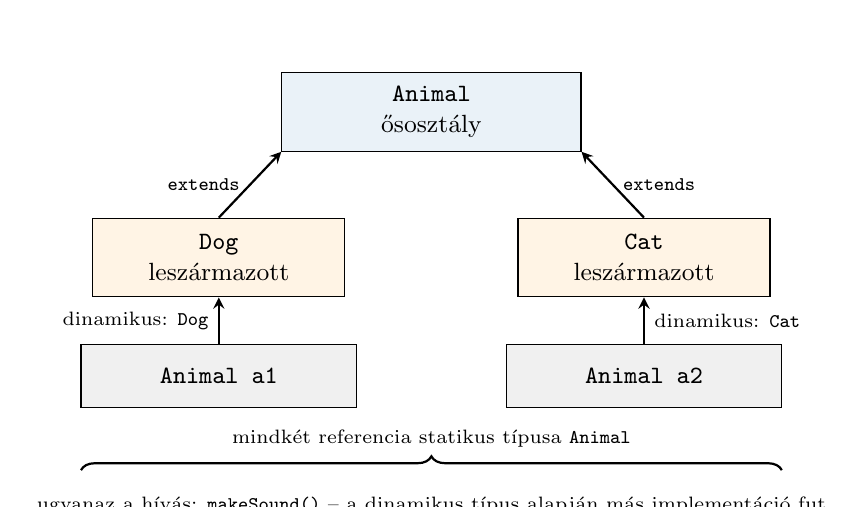
\begin{tikzpicture}[font=\small]
  \node[zvflowprocess, fill=lightaccent, minimum width=38mm, minimum height=10mm] (animal) at (0,2.3) {\texttt{Animal}\\ ősosztály};

  \node[zvflowprocess, fill=warnbg, minimum width=32mm, minimum height=10mm] (dog) at (-2.7,0.45) {\texttt{Dog}\\ leszármazott};
  \node[zvflowprocess, fill=warnbg, minimum width=32mm, minimum height=10mm] (cat) at (2.7,0.45) {\texttt{Cat}\\ leszármazott};

  \node[zvflowprocess, fill=black!6, minimum width=35mm, minimum height=8mm] (ref1) at (-2.7,-1.05) {\texttt{Animal a1}};
  \node[zvflowprocess, fill=black!6, minimum width=35mm, minimum height=8mm] (ref2) at (2.7,-1.05) {\texttt{Animal a2}};

  \draw[arrow] (dog.north) -- node[left,font=\scriptsize] {\code{extends}} (animal.south west);
  \draw[arrow] (cat.north) -- node[right,font=\scriptsize] {\code{extends}} (animal.south east);

  \draw[arrow] (ref1) -- node[left,font=\scriptsize] {dinamikus: \texttt{Dog}} (dog);
  \draw[arrow] (ref2) -- node[right,font=\scriptsize] {dinamikus: \texttt{Cat}} (cat);

  \node[align=center, font=\scriptsize] at (0,-1.85) {mindkét referencia statikus típusa \texttt{Animal}};
  \draw[decorate, decoration={brace, amplitude=5pt}, thick] (-4.45,-2.25) -- node[below=6pt, font=\scriptsize, align=center] {ugyanaz a hívás: \texttt{makeSound()} -- a dinamikus típus alapján más implementáció fut} (4.45,-2.25);
\end{tikzpicture}
\caption{Öröklődés és polimorfizmus: ősosztály típusú referencia, eltérő dinamikus típus}
\label{fig:zv15_oroklodes_polimorfizmus}
\end{figure}


\zvcode[language=Java,caption={Öröklődés, statikus/dinamikus típus és polimorf metódushívás},label={lst:zv15_inheritance_polymorphism}]{src/code/zv15_inheritance_polymorphism.java}

A példában a \code{first} és \code{second} változó statikus típusa egyaránt \code{Animal}. A dinamikus típusuk viszont eltérő: az egyik \code{Dog}, a másik \code{Cat}. Emiatt a \code{makeSound()} hívás ugyanazzal a statikus típussal más implementációhoz vezet.

\section{Polimorfizmus}

\subsection{A polimorfizmus fogalma}

A \textbf{polimorfizmus} szó szerint többalakúságot jelent. Objektumorientált programozásban azt jelenti, hogy ugyanaz az üzenet vagy metódushívás különböző objektumokon különböző módon hajtódhat végre. A felhasználó kód általános típust lát, a konkrét viselkedést pedig a tényleges objektum osztálya adja.

A tétel szempontjából két fontos forma különíthető el:

\begin{itemize}
  \item \textbf{ad-hoc vagy fordításidejű polimorfizmus}: metódustúlterhelés, ahol a fordító választ a szignatúrák között;
  \item \textbf{szubtípus-polimorfizmus}: ősosztály vagy interfész típusú referencia mögött többféle leszármazott objektum állhat.
\end{itemize}

Vizsgán a hangsúly általában a szubtípus-polimorfizmuson van, mert ez kapcsolja össze az öröklődést, a felüldefiniálást, az absztrakt osztályokat és az interfészeket.

\subsection{Polimorf kód előnye}

Polimorf kódban a vezérlő logika nem konkrét osztályokra épül, hanem általános felületre. Például ha minden alakzatnak van \code{area()} metódusa, akkor egy területszámító algoritmusnak nem kell külön vizsgálnia, hogy az objektum kör, téglalap vagy háromszög. Elég az absztrakt \code{Shape} típus vagy egy megfelelő interfész.

Ennek előnyei:

\begin{itemize}
  \item kisebb függés konkrét osztályoktól;
  \item könnyebb bővíthetőség új leszármazottakkal;
  \item áttekinthetőbb, általánosabb algoritmusok;
  \item egységes kezelés különböző objektumokra.
\end{itemize}

\subsection{Upcast és downcast}

\textbf{Upcast} esetén egy leszármazott objektumot ősosztály vagy interfész típusú referenciával kezelünk. Ez biztonságos és automatikus:

\[
  \code{Animal animal = new Dog("Morzsa");}
\]

\textbf{Downcast} esetén egy általánosabb típusú referenciát konkrétabb típusra alakítunk vissza:

\[
  \code{Dog dog = (Dog) animal;}
\]

Ez csak akkor helyes, ha az objektum dinamikus típusa valóban \code{Dog} vagy annak leszármazottja. Ha nem, akkor futásidőben \code{ClassCastException} keletkezik. Biztonságosabb megoldás az \code{instanceof} használata, ha tényleg szükség van konkrét típusfüggő műveletre.

\section{Absztrakt osztály}

\subsection{Fogalma és szerepe}

Az \textbf{absztrakt osztály} olyan osztály, amelyet közvetlenül nem lehet példányosítani. Célja, hogy közös alapot adjon a leszármazott osztályoknak. Tartalmazhat konkrét mezőket, konstruktorokat és megvalósított metódusokat, de tartalmazhat absztrakt metódusokat is.

Absztrakt metódus esetén csak a metódus fejét adjuk meg, implementáció nélkül. Az absztrakt metódus azt jelenti, hogy a konkrét leszármazott osztályoknak kell megadniuk a viselkedést. Ha egy osztály nem valósítja meg az összes örökölt absztrakt metódust, akkor maga is absztrakt marad.

Java-ban az absztrakt osztály jelölése:

\[
  \code{abstract class Shape \{ ... \}}
\]

Absztrakt metódus példája:

\[
  \code{public abstract double area();}
\]

\subsection{Mikor célszerű absztrakt osztályt használni?}

Absztrakt osztályt akkor érdemes használni, ha a leszármazottak között valódi rokonság van, és közös kódot vagy közös állapotot is meg akarunk osztani. Például minden \code{Shape} alakzatnak lehet közös \code{color} mezője és \code{describe()} metódusa, miközben az \code{area()} kiszámítása alakzatonként eltérő.

Az absztrakt osztály tehát részleges implementáció: egyszerre adhat közös működést és kötelezően megvalósítandó műveleteket.

\section{Interfész}

\subsection{Fogalma és szerepe}

Az \textbf{interfész} olyan típus, amely szerződést ír elő. Megmondja, hogy az interfészt megvalósító osztályoknak milyen műveleteket kell biztosítaniuk. Java-ban az interfészt az \code{interface} kulcsszóval definiáljuk, az osztály pedig az \code{implements} kulcsszóval valósítja meg.

Például egy \code{Drawable} interfész azt fejezheti ki, hogy az objektum kirajzolható:

\[
  \code{interface Drawable \{ void draw(); \}}
\]

Egy osztály több interfészt is megvalósíthat. Ez azért fontos, mert Java-ban osztályok között nincs többszörös öröklődés, de interfészeken keresztül egy objektum több szerepet vagy képességet is vállalhat. Például egy \code{Circle} lehet egyszerre \code{Shape}, \code{Drawable} és \code{Scalable}.

\subsection{Interfész mint polimorf felület}

Az interfész egyik legfontosabb szerepe a laza csatolás. Ha egy metódus \code{Drawable} típusú paramétert vár, akkor nem kell tudnia, hogy a konkrét objektum \code{Circle}, \code{Button}, \code{Icon} vagy más típus. Csak az számít, hogy rendelkezzen \code{draw()} metódussal.

Ez különösen hasznos nagyobb rendszerekben, mert a kód nem konkrét implementációktól függ, hanem szerződésektől. Így könnyebb tesztelni, cserélni és bővíteni az egyes részeket.

\section{Absztrakt osztály és interfész összehasonlítása}

Az absztrakt osztály és az interfész is absztrakt típus: egyikből sem hozunk létre közvetlen objektumot, viszont referenciatípusként mindkettő használható. Mindkettő segíti a polimorfizmust, mert a konkrét objektumokat általánosabb típuson keresztül kezelhetjük.

A különbség főleg a szerepükben van. Az absztrakt osztály közös alapot és részleges implementációt ad rokon osztályoknak. Az interfész inkább képességet, protokollt vagy szerződést ír le, és több, egymástól független osztály is megvalósíthatja.

\begin{center}
\begin{tabularx}{\textwidth}{L{32mm}X X}
\toprule
\textbf{Szempont} & \textbf{Absztrakt osztály} & \textbf{Interfész} \\
\midrule
Szerep & Közös alap és részleges implementáció megadása rokon osztályoknak. & Szerződés megadása arról, hogy egy típus milyen műveleteket biztosít. \\
Példányosítás & Közvetlenül nem példányosítható. & Közvetlenül nem példányosítható. \\
Állapot & Tartalmazhat példánymezőket és konstruktorokat. & Általában nem objektumállapot tárolására való; konstansokat tartalmazhat. \\
Metódusok & Lehetnek absztrakt és konkrét metódusai is. & Tartalmazhat absztrakt metódusokat, valamint Java 8 óta \code{default} és \code{static} metódusokat is. \\
Öröklési korlát & Egy osztály csak egy közvetlen osztályból örökölhet. & Egy osztály több interfészt is megvalósíthat. \\
Használati helyzet & Akkor célszerű, ha közös kódot és közös állapotot is meg akarunk osztani. & Akkor célszerű, ha képességet, protokollt vagy szerepet akarunk leírni lazább csatolással. \\
Kulcsszavak & \code{abstract class}, \code{extends}. & \code{interface}, \code{implements}. \\
\bottomrule
\end{tabularx}

\end{center}

\zvcode[language=Java,caption={Absztrakt osztály és interfészek együtt használva},label={lst:zv15_abstract_interface}]{src/code/zv15_abstract_interface.java}

A példában a \code{Shape} absztrakt osztály közös állapotot és közös metódust ad, az \code{area()} metódus implementációját viszont a konkrét alakzatokra bízza. A \code{Drawable} és \code{Scalable} interfészek képességeket írnak le: egy objektum kirajzolható, illetve skálázható lehet.

\section{Gyakori félreértések}

\subsection{A túlterhelés nem ugyanaz, mint a felüldefiniálás}

A túlterhelésnél azonos nevű, de eltérő paraméterlistájú metódusokról van szó. A fordító a statikus típusok és az argumentumok alapján választ. Felüldefiniálásnál viszont az örökölt metódus új implementációjáról van szó, és a választás futásidőben, a dinamikus típus alapján történik.

\subsection{A \code{private} tag nem polimorf bővítési pont}

A \code{private} metódust a leszármazott nem definiálja felül, mert az nem látható örökölt metódusként. Ha a leszármazottban ugyanilyen nevű metódust írunk, az egy új, külön metódus lesz. Polimorf működéshez elérhető, felüldefiniálható példánymetódus kell.

\subsection{A statikus típus korlátozza, mit hívhatunk meg}

Ha egy \code{Dog} objektumot \code{Animal} típusú referencián keresztül kezelünk, akkor a fordító csak az \code{Animal} típusban ismert tagokat engedi meghívni. A dinamikus típus a felüldefiniált metódus kiválasztásánál számít, nem általános jogosultság arra, hogy bármilyen \code{Dog}-specifikus metódust meghívjunk.

\subsection{Az interfész nem pusztán üres osztály}

Az interfész nem osztály, hanem szerződés. Nem az a fő célja, hogy közös állapotot tároljon, hanem az, hogy egységesen előírjon bizonyos műveleteket. Egy osztály több interfészt is megvalósíthat, ezért az interfészek alkalmasak többféle szerep kifejezésére.

\subsection{Az öröklés nem mindig jobb, mint a kompozíció}

Sok kezdő hiba abból ered, hogy minden kapcsolatot öröklődéssel próbálnak modellezni. Ha az egyik objektum csak használja vagy tartalmazza a másikat, akkor gyakran jobb megoldás a kompozíció. Öröklődést akkor célszerű alkalmazni, ha valódi specializációról van szó.

\section{Tipikus vizsgakérdések és rövid válaszvázlatok}

\subsection{Mit jelent az öröklődés?}

Az öröklődés az OOP egyik alapelve, amelyben egy leszármazott osztály egy meglévő ősosztály specializációjaként jön létre. A leszármazott örökli az ős elérhető tagjait, új tagokat vehet fel, és felüldefiniálhat örökölt metódusokat. Java-ban az osztályöröklés kulcsszava az \code{extends}, és egy osztálynak csak egy közvetlen ősosztálya lehet.

\subsection{Mi a különbség a túlterhelés és a felüldefiniálás között?}

Túlterhelésnél azonos nevű, de eltérő paraméterlistájú metódusok vannak, és a választás fordítási időben történik. Felüldefiniálásnál a leszármazott osztály új implementációt ad az ősosztály azonos szignatúrájú példánymetódusára, és a ténylegesen futó implementációt a dinamikus típus alapján választja ki a rendszer.

\subsection{Mit jelent a statikus és dinamikus típus?}

A statikus típus a referencia deklarált, fordításkor ismert típusa. Ez határozza meg, milyen tagokat enged meghívni a fordító. A dinamikus típus a futásidőben ténylegesen létrejött objektum konkrét osztálya. Felüldefiniált példánymetódus hívásakor a dinamikus típus dönti el, melyik implementáció fut le.

\subsection{Mi az absztrakt osztály szerepe?}

Az absztrakt osztály közvetlenül nem példányosítható. Közös alapot ad leszármazott osztályoknak: tartalmazhat közös állapotot, konstruktorokat, konkrét metódusokat és absztrakt metódusokat is. Akkor célszerű használni, ha rokon osztályok között közös kódot vagy közös állapotot is meg akarunk osztani.

\subsection{Mi az interfész szerepe?}

Az interfész szerződést ír elő: megadja, hogy az azt megvalósító osztálynak milyen műveleteket kell biztosítania. Interfészen keresztül a kód nem konkrét implementációtól, hanem képességtől vagy protokolltól függ. Java-ban egy osztály több interfészt is megvalósíthat, ezért az interfész fontos eszköz a rugalmas, polimorf tervezéshez.

\section{Összefoglalás vizsgára}

\begin{summarybox}
Az öröklődés az általánosabb osztályból speciálisabb osztály létrehozásának eszköze. Java-ban osztályok között egyszeres öröklődés van, az \code{extends} kulcsszóval. A leszármazott örökli az ős elérhető tagjait, de a konstruktorokat nem; az ős konstruktorát \code{super(...)} hívással lehet elérni. A túlterhelés azonos nevű, eltérő paraméterlistájú metódusokat jelent, és fordítási időben dől el. A felüldefiniálás örökölt példánymetódus új implementációja, amely polimorf hívásnál futásidőben, a dinamikus típus alapján választódik ki. A statikus típus a deklarált típus, a dinamikus típus a tényleges objektumtípus. Az absztrakt osztály közös részleges implementációt és absztrakt műveleteket adhat, az interfész pedig szerződést, képességet vagy szerepet ír le. Mindkettő használható polimorf referenciatípusként.
\end{summarybox}

\end{document}
